\documentclass[11pt]{article}
\usepackage[T1]{fontenc}
\usepackage[utf8]{inputenc}
\usepackage{lmodern,amsmath,amssymb,amsthm,mathtools,mathrsfs,graphicx,xcolor}
\usepackage[a4paper,margin=24mm]{geometry}
\usepackage{microtype}
\usepackage[colorlinks=true,hypertexnames=false,linkcolor=blue!50!black,urlcolor=blue!50!black]{hyperref}
\setlength{\emergencystretch}{3em}
\allowdisplaybreaks
\title{Full Weil positivity and the surviving mixed-support trace\\
\large Exact prime energies and the original companion boundary}
\author{Programme continuation with explicit source provenance}
\date{23 September 2026 --- SZ-20260923-033}
\begin{document}
\maketitle

This continuation receives the actual degree-$p$ operator on the
relative principal parts and computes its action on the original
mixed-support tests. The resulting signed joint observation admits
both signs even on compact convolution squares satisfying both Weil
moments. We then evaluate the full Archimedean term and prove that
the entire three-pulse family has strictly positive complete Weil
form, with the exact lower bound $5981N/52500$. These tests are
therefore excluded as full-Weil counterexamples. Their mixed support
state remains nonzero; after retaining the common Archimedean term,
its joint trace is strictly negative at every tensor order at least
two. The complete maps and proofs of these assertions follow.

The companion calculation constructs the original off-critical
$q$-dimensional object as a recurrence subspace in the actual
local tensor operator's annulus distribution channel. It retains
every original cardinal label, phase, source metric, support label
and observation-kernel component. Evaluation at zero is its exact
inverse. Its exponential growth and its two finite boundary terms
are calculated without identifying that distribution subspace with
the global interior cohomology. No RH decision is claimed.

\paragraph{Human sources and programme inputs.}
The analytic convention is Alain Connes's original author TeX,
\href{https://arxiv.org/abs/2602.04022v1}{\emph{The Riemann Hypothesis:
Past, Present and a Letter Through Time}}, section
\texttt{sectweilpos}, equations \texttt{wp} and \texttt{arch},
which attributes the positivity criterion to Andr\'e Weil.
The source of the relative principal parts and local degree operator
is the supplied 031 proof, RP21--38, PD1--21 and IA1--9.
The full-lattice carrier, original companion coordinates and mixed
support diagonal are the supplied 032 proof, CLM8--17, CR1--41,
PDD1--15, JMD1--23 and TDP1--4. Their complete, exact-version TeX
sources accompany this paper in the reproducibility archive,
under \texttt{inputs/031\_SOURCE.tex} and
\texttt{inputs/032\_SOURCE.tex}; the source account records their
hashes. These supplied witnesses are identified as such, with no
unverified public-edition claim. The full local operator proofs and
all input definitions needed for the new assertions are included
again where used below.

The supported-zero prime chain is prior foundational work. The
user-provided origin attribution is Gemini 2.5 Pro; the first
\href{https://github.com/KokunoYumeto/zeta-function-research-reader/blob/d2f0020a7c446f429682925c1c682d99ba86a4cc/workbenches/splitzero-tandem/foundations/globalization-semiring/globalization_note.tex#L239}{globalization source, prime-ideal classification and dimension corollary},
has an empty author field, while the later full-lattice Version 11
has the byline The Clankers. These identities are not merged.
The general purity comparison belongs to Pierre Deligne,
\href{https://www.numdam.org/item/PMIHES_1980__52__137_0/}{\emph{La
conjecture de Weil. II}}, especially 3.3.6 for the image of compactly
supported cohomology in ordinary cohomology. No application of
that theorem to the constructed annulus space is assumed here.
The proofs below do not require an unverified transcription of
Deligne's theorem. Earlier ES--Fable provenance remains with its
original Levent Alp\"oge credit in the retained input collection;
no new ES result is asserted in this continuation.

\clearpage
\tableofcontents
\clearpage
\begin{figure}[p]
\centering
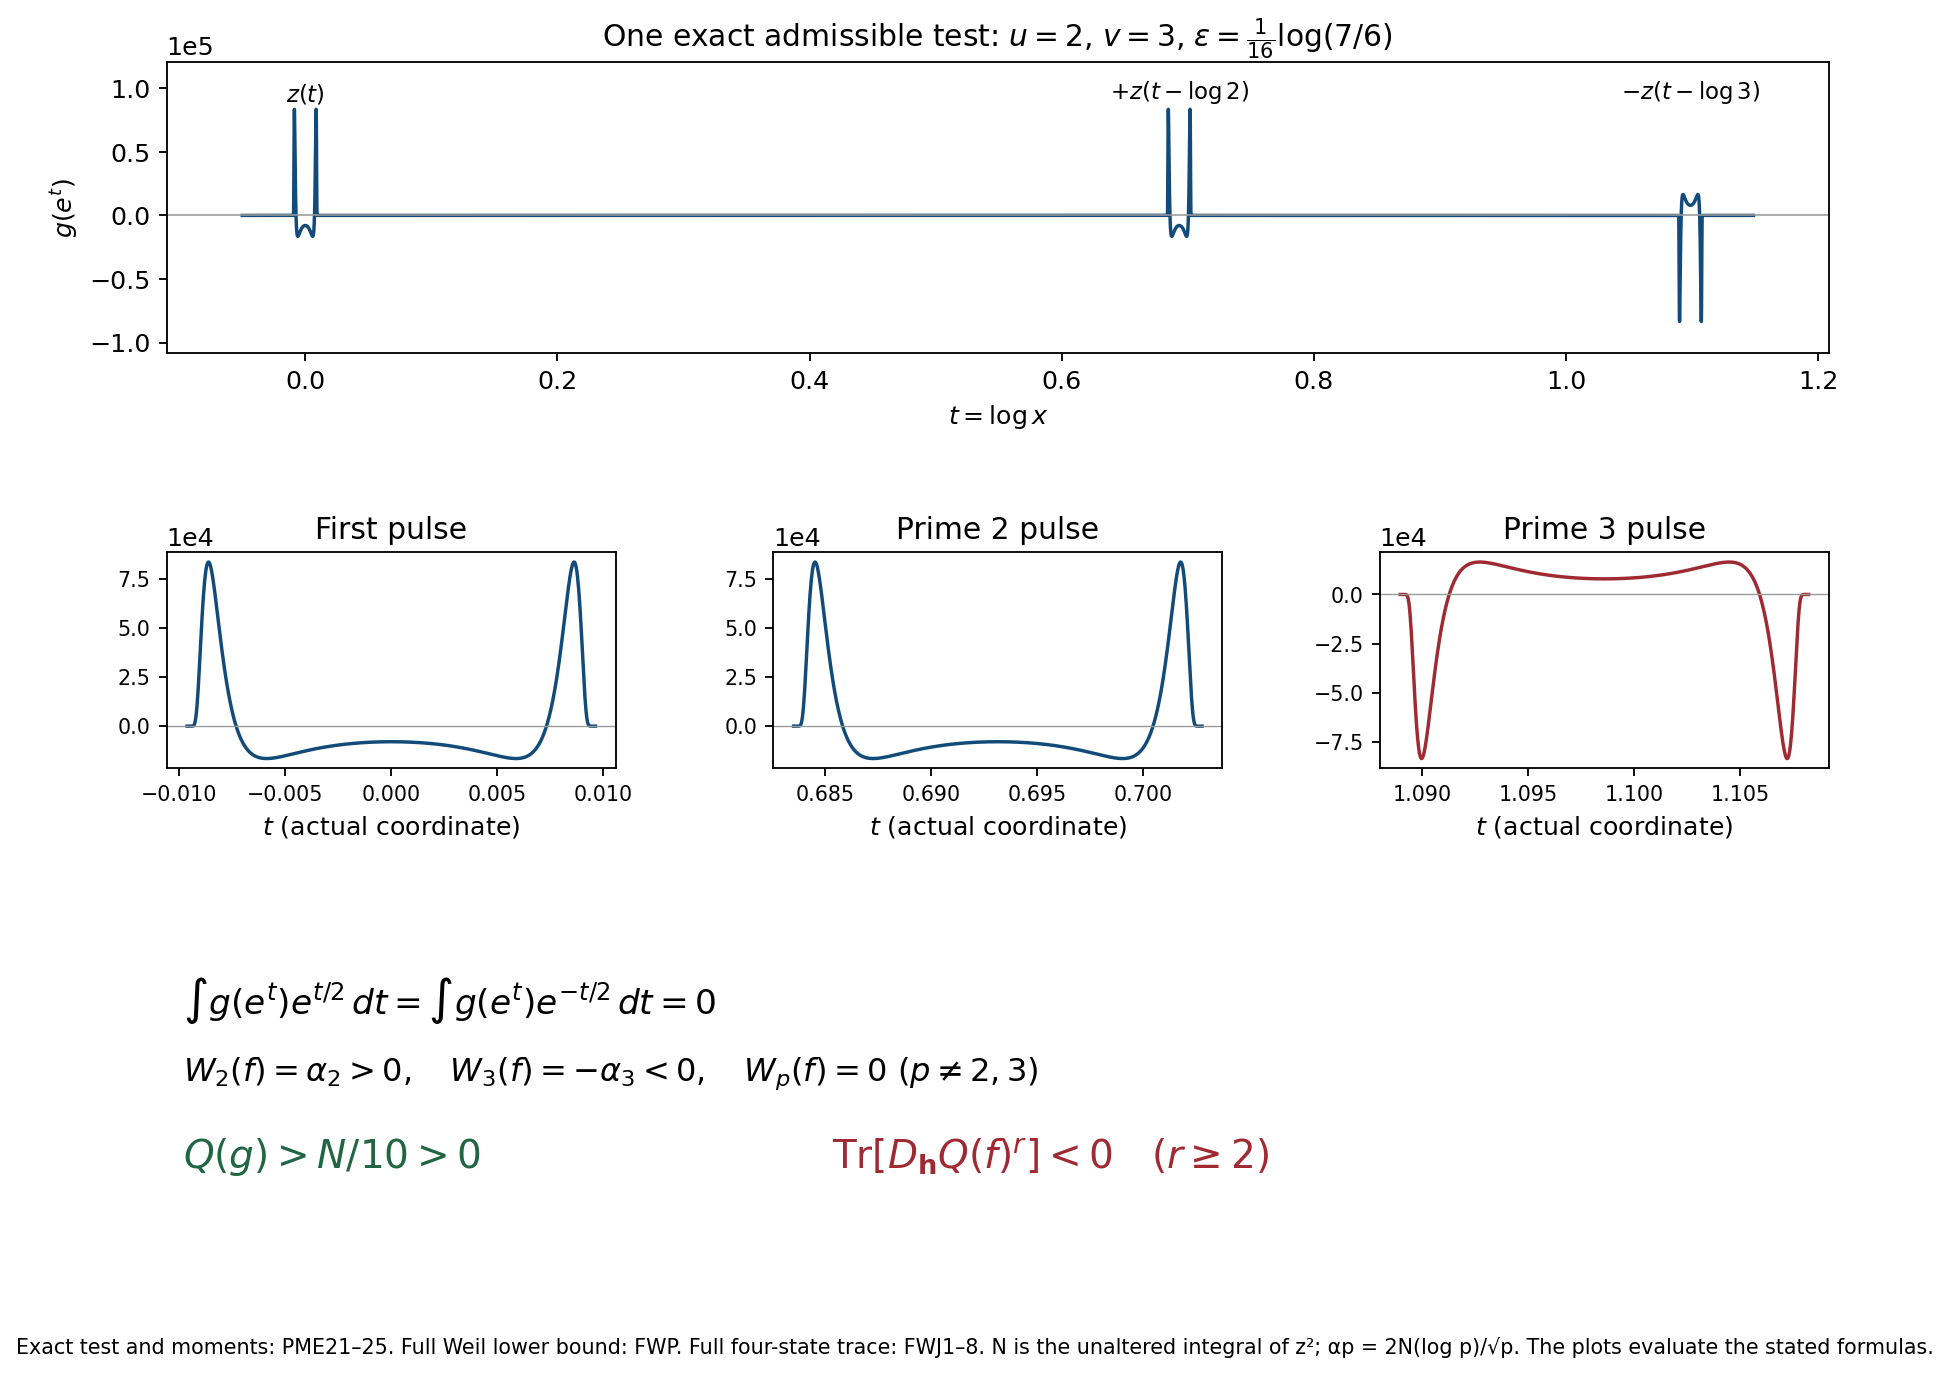
\includegraphics[width=\linewidth]{ADMISSIBLE_MIXED_TEST.png}
\caption{The actual three-pulse test for primes 2 and 3, in its original
logarithmic coordinate and amplitude. PME21--25 proves both Mellin
conditions and every prime evaluation; FWP1--24 proves the complete
Weil lower bound with Connes's full Archimedean term. FWJ1--8 proves
the simultaneously negative signed support trace, including that
same Archimedean term. The expanded pulse panels show the indicated
coordinate intervals without changing the pulse amplitudes.}
\end{figure}
\clearpage
% Complete independent mathematical derivation. Equation prefix PME.
% Companion sources: SZ-20260922-031 PD1--21, RP36--38, IA1--9;
% SZ-20260922-032 PDD1--15 and JMD1--23. No sealed source was edited.
\section{The relative prime degree on admissible mixed-support tensors}
\label{sec:prime-degree-mixed-admissible}

The calculation in this section composes the actual prime-degree
operator of the 031 continuation with the compact tests and the
support diagonal of the 032 continuation. It establishes both signs
for their mixed observation on genuine admissible convolution squares.
The complete Weil sign for the constructed three-pulse family is
calculated in Section~\ref{sec:full-weil-three-pulse}.

\paragraph{Sources, authorship, and scope.}
The prior inputs are the programme's 031 working source
\texttt{01\_REBUILT\_MATHEMATICS.tex}, equations PD1--PD21,
RP36--RP38, and IA1--IA9, and the 032 working source, equations
PDD1--PDD15 and JMD1--JMD23. The new computation is the exact
composition proved below. The finite-place distributions and
Mellin convention are Alain Connes's original author TeX,
\href{https://arxiv.org/abs/2602.04022v1}{\emph{The Riemann
Hypothesis: Past, Present and a Letter Through Time}},
section \texttt{sectweilpos}, equation \texttt{wp}; that section
attributes the positivity criterion to Andr\'e Weil.
The supported-zero foundation is an earlier programme result, not a
discovery of this calculation. The user's attribution of its original
derivation to Gemini 2.5 Pro is retained separately from the supplied
original source's empty author field and the later Version 11 byline
The Clankers. Its exact original source is
\href{https://github.com/KokunoYumeto/zeta-function-research-reader/blob/d2f0020a7c446f429682925c1c682d99ba86a4cc/workbenches/splitzero-tandem/foundations/globalization-semiring/globalization_note.tex#L298}{\texttt{globalization\_note.tex}, supported-zero prime theorem}.
No class-semigroup claim is used here.

\subsection{Independent verification of the prime-degree receiver}

Fix a rational prime $p$. Retain $|p|_p=p^{-1}$ and additive Haar
measure $\mu(\mathbb Z_p)=1$. Put
$D_p=\mathbb Z[1/p]/\mathbb Z=\mathbb Q_p/\mathbb Z_p$.
The equality is the map induced by rational inclusion: its kernel is
zero because $a/p^n\in\mathbb Z_p$ implies $p^n\mid a$, and its
surjectivity follows by taking the finite negative part of a $p$-adic
expansion. Multiplication by $p$ on $D_p$ is onto and has exactly
$p$ elements in every fibre; its kernel consists of the classes $a/p$.
On counting-measure $\ell^2(D_p)$ the actual pullback and its adjoint are
\[
 (A_pf)(d)=f(pd),\qquad
 (A_p^*f)(u)=\sum_{pd=u}f(d),\qquad A_p^*A_p=pI.
 \tag{PME1}
\]
These formulas first hold on finite-support functions. Fibre counting
gives $\|A_pf\|^2=p\|f\|^2$, so they extend boundedly and
$V_p=p^{-1/2}A_p$ is an isometry. Its factor is fixed by the degree.

For $d=a/p^n$ define
$\chi_d(x)=\exp(2\pi i a(x\bmod p^n)/p^n)$ on $\mathbb Z_p$.
Changing representatives or increasing $n$ leaves the character
unchanged. The finite geometric sum proves orthogonality of these
characters for Haar measure one. At each level they are a basis of
the functions on $\mathbb Z/p^n\mathbb Z$, and those functions
are dense in $L^2(\mathbb Z_p)$. Thus
$\delta_d\mapsto\chi_d$ is unitary. Under this Fourier convention,
\[
 V_pF(x)=\sqrt p\,\mathbf1_{p\mathbb Z_p}(x)F(x/p),
 \qquad V_p^*F(x)=p^{-1/2}F(px).
 \tag{PME2}
\]
Indeed the sum of $\chi_d(x)$ over $pd=u$ vanishes unless
$x\in p\mathbb Z_p$, and for $x=py$ it is $p\chi_u(y)$.
Changing variables $x=py$, $dx=p^{-1}dy$, proves the adjoint.
The range projection of $V_p^n$ is multiplication by
$\mathbf1_{p^n\mathbb Z_p}$, whose decreasing ranges have zero
intersection because the limiting singleton has Haar measure zero.

On $\mathscr H_p=L^2(\mathbb Q_p)$ define
\[
 (\mathscr U_pF)(x)=\sqrt p F(x/p),\quad
 (\mathscr U_p^{-1}F)(x)=p^{-1/2}F(px),\quad
 \xi_p=\mathbf1_{\mathbb Z_p},\quad r_p=p^{-1/2}.
 \tag{PME3}
\]
The change of variables above proves unitarity. Extension by zero
embeds the space in PME2 and intertwines its isometry with
$\mathscr U_p$. The spaces supported in $p^{-n}\mathbb Z_p$
exhaust $\mathscr H_p$, so this is the minimal unitary extension.
For $n\ge0$, $\mathscr U_p^n\xi_p=p^{n/2}\mathbf1_{p^n\mathbb Z_p}$.
Integration, and then unitarity for negative $n$, give
\[
 \langle\mathscr U_p^n\xi_p,\xi_p\rangle=r_p^{|n|},\qquad
 d\nu_p(\theta)=\frac{1}{2\pi}
 \frac{1-r_p^2}{1-2r_p\cos\theta+r_p^2}\,d\theta.
 \tag{PME4}
\]
The measure assertion follows by summing the two absolutely convergent
geometric series and then expanding the squared norm of every
Laurent polynomial applied to $\xi_p$. These polynomial pairings
determine the cyclic measure by density of trigonometric polynomials.

For precision the actual weight-one operator is
$T_p^{\rm rel}=\sqrt p\mathscr U_p$, not the isometry $V_p$.
It satisfies
\[
 (T_p^{\rm rel})^*T_p^{\rm rel}
 =T_p^{\rm rel}(T_p^{\rm rel})^*=pI,
 \qquad \sigma(T_p^{\rm rel})=\{z:|z|=\sqrt p\}.
 \tag{PME5}
\]
To prove the entire spectrum assertion, the annuli
$p^n\mathbb Z_p^\times$, $n\in\mathbb Z$, partition
$\mathbb Q_p$ outside a null singleton. Their $L^2$ spaces are the
mutually orthogonal translates of $L^2(\mathbb Z_p^\times)$ by
$\mathscr U_p^n$. On this direct sum $\mathscr U_p$ is the
bilateral shift. For a unit vector $b$ in the zeroth summand and
$|\lambda|=1$, the unit vectors
$(2N+1)^{-1/2}\sum_{n=-N}^N\lambda^{-n}\mathscr U_p^n b$
have squared $(\mathscr U_p-\lambda)$-error $2/(2N+1)$.
For $|\lambda|\ne1$ a Neumann series for $\mathscr U_p$ or its
inverse gives the inverse of $\mathscr U_p-\lambda$.
This proves PME5 after scaling. An eigenvector would have equally
large components in all annular summands, so square summability
forces every component to vanish. There are no nonzero eigenvectors.
These checks validate PD1--PD13 and PD20--PD21 with their stated
measures, Fourier signs, and distinctions between the operators.

\subsection{The exact bounded energy map and its signed operator}

Let $H=L^2(\mathbb R_+^\times,dx/x)$, with inner product linear
in the first variable. For $g\in C_c^\infty(\mathbb R_+^\times)$
put $F(t)=g(e^t)$, $a_p=\log p$, and retain the actual map
\[
 (\mathcal E_pg)(x)=\sum_{n\in\mathbb Z}
 F(x+na_p)\mathscr U_p^n\xi_p,\qquad 0\le x<a_p,
 \quad
 \mathcal E_p:H\longrightarrow
 K_p:=L^2([0,a_p);\mathscr H_p).
 \tag{PME6}
\]
The sum is finite on the initial domain. Write
$g^*(x)=\overline{g(x^{-1})}$ and
$f=g*g^*$, using Haar convolution $dx/x$.
Expanding the norm and applying PME4, then setting $j=n-m$ and
$t=x+na_p$, proves
\[
 \begin{split}
 \|\mathcal E_pg\|^2
 &=\sum_{j\in\mathbb Z}r_p^{|j|}
       \int_{\mathbb R} F(t)\overline{F(t-ja_p)}\,dt\\
 &=\frac1{2\pi}\int_{\mathbb R}|\widehat g(s)|^2
       P_{r_p}(a_ps)\,ds,
 \qquad
 P_r(\theta)=\frac{1-r^2}{1-2r\cos\theta+r^2},
 \quad \widehat g(s)=\int_0^\infty g(x)x^{-is}\,\frac{dx}{x}.
 \end{split}
 \tag{PME7}
\]
For fixed $j$ the intervals in the change of variables partition
$\mathbb R$ up to endpoints. Fourier inversion gives the second
line. Interchange with the Poisson series is justified by its
absolute sum $(1+r_p)/(1-r_p)$ times the integrable function
$|\widehat g(s)|^2$. Consequently PME6 extends uniquely boundedly,
with $\|\mathcal E_p\|^2=(1+r_p)/(1-r_p)$: the upper bound follows
from PME7 and is attained as a supremum by functions whose Fourier
mass is supported near $s=0$, where $P_{r_p}$ attains its maximum.
Polarization of PME7 identifies the bounded self-adjoint operator
\[
 B_p=(\log p)(\mathcal E_p^*\mathcal E_p-I_H)
 \quad\hbox{with multiplier}\quad
 b_p(s)=(\log p)(P_{r_p}(a_ps)-1).
 \tag{PME8}
\]
Its exact range, hence its essential range and spectrum, is
\[
 \sigma(B_p)=
 \left[-\frac{2r_p\log p}{1+r_p},
         \frac{2r_p\log p}{1-r_p}\right].
 \tag{PME9}
\]
The denominator of $P_r$ ranges continuously from $(1-r)^2$ to
$(1+r)^2$. Every neighborhood of each attained value has a preimage
of positive Lebesgue measure. Multiplication by $b_p-z$ has bounded
inverse outside the closed range, while supported unit vectors near
any value in the range are approximate eigenvectors. This proves
PME9 without transferring an unproved spectral assertion.

The $j=0$ summand of PME7 is $\|g\|^2$. Hence the entire
prime-power distribution in Connes's stated convention is
\[
 W_p(f)=(\log p)\sum_{m\ge1}p^{-m/2}
                  [f(p^m)+f(p^{-m})]
       =\langle B_pg,g\rangle
       =(\log p)(\|\mathcal E_pg\|^2-\|g\|^2).
 \tag{PME10}
\]
This verifies PD14--PD17 and their signs. It also agrees with
RP36--RP38: the trace-class diagonal operator
$D_p(s)e_m=p^{-ms}e_m$, $m\ge1$, has trace
$\sum_{m\ge1}p^{-ms}$ for $\Re s>0$. Substituting
$s=1/2\pm it$ into both traces and using Fourier inversion gives
exactly PME10, including $1/(2\pi)$ and every $\log p$.
The sum of absolute trace coefficients is $2r_p/(1-r_p)$,
which justifies the integral interchange. Similarly the scalar
resolvent on $\xi_p$ is $(1-zr_p)^{-1}$ for $|z|<1$;
its scalar series extends to $|z|<\sqrt p$ without an operator
resolvent assertion there. This verifies PD19's stated distinction.

The calculation exhibits why PME5 alone does not make PME10
nonnegative: the exact receiving map subtracts $I_H$, and its
operator has both signs by PME9. No local degree or measure factor
is changed in this statement.

\subsection{Composition with the original PDD tests}

Retain every PDD coefficient. For each prime $p$, set
\[
 \begin{gathered}
 \varepsilon_p=\tfrac18\log((p+1)/p),\qquad
 u_p(t)=
 \begin{cases}e^{-1/(1-(t/\varepsilon_p)^2)},&|t|<\varepsilon_p,\\
 0,&|t|\ge\varepsilon_p,
 \end{cases}\\
 v_p=u_p''-\tfrac14u_p,\quad
 N_p=\int_{\mathbb R}|v_p(t)|^2dt.
 \end{gathered}
 \tag{PME11}
\]
Every derivative of the bump tends to zero at the endpoints,
because the exponential dominates each inverse power of
$1-(t/\varepsilon_p)^2$. Thus the displayed functions are smooth.
Integration by parts gives
$\int v_pu_p=-\int|u_p'|^2-\tfrac14\int u_p^2<0$, so $N_p>0$.
For $\sigma\in\{1,-1\}$ put
\[
 g_{p,\sigma}(e^t)=v_p(t)+\sigma v_p(t-a_p),\qquad
 f_{p,\sigma}=g_{p,\sigma}*g_{p,\sigma}^*.
 \tag{PME12}
\]
Two integrations by parts, including their zero boundary terms, give
$\int v_p(t)e^{ct}dt=(c^2-1/4)\int u_p(t)e^{ct}dt=0$
for $c=1/2$ and $c=-1/2$. Translation multiplies this zero by
$e^{ca_p}$. Therefore both original Mellin values of $g_{p,\sigma}$
at $\pm i/2$ vanish.

Let $C_p(b)=\int v_p(t)v_p(t-b)dt$. It is even, supported in
$[-2\varepsilon_p,2\varepsilon_p]$, and $C_p(0)=N_p$.
Expanding the convolution gives
$f_{p,\sigma}(e^b)=2C_p(b)+\sigma C_p(b-a_p)+\sigma C_p(b+a_p)$.
For every integer $n\ge2$, $n\ne p$,
$|\log n-a_p|\ge\log((p+1)/p)=8\varepsilon_p$;
below $p$ use $p/(p-1)>(p+1)/p$, and above $p$ use monotonicity.
Also $2\varepsilon_p<\log2$ and $2\varepsilon_p<a_p$.
These facts prove all the evaluations, and their energy receivers,
\[
 \begin{split}
 \|g_{p,\sigma}\|^2&=2N_p,\\
 W_q(f_{p,\sigma})&=2\sigma(\log p)r_pN_p\,\mathbf1_{q=p},\\
 \|\mathcal E_qg_{p,\sigma}\|^2
   &=2N_p(1+\sigma r_p\mathbf1_{q=p}).
 \end{split}
 \tag{PME13}
\]
Here unique factorization ensures $q^m=p$ only for $q=p,m=1$.
The last line follows by the proved PME10; it computes the actual
energy map for every prime, not only the chosen one.

There is also a direct vector calculation at $q=p$:
\[
 (\mathcal E_pg_{p,\sigma})(x)=
 \begin{cases}
 v_p(x)(\xi_p+\sigma\mathscr U_p\xi_p),&0\le x<\varepsilon_p,\\
 v_p(x-a_p)(\mathscr U_p^{-1}\xi_p+\sigma\xi_p),
       &a_p-\varepsilon_p<x<a_p,\\
 0,&\varepsilon_p\le x\le a_p-\varepsilon_p.
 \end{cases}
 \tag{PME14}
\]
Each nonzero case comes from exactly two terms of PME6. Both vector
norms squared are $2(1+\sigma r_p)$ by PME4, and the two integrals
of $v_p^2$ add to $N_p$. This independently verifies its PME13 value.

\subsection{The two-place support trace and all four signed energies}

Fix distinct rational primes $u,v$. In the four-state space
$V=\mathbb C[\mathcal P(\{u,v\})]$, retain
\[
 \mathbf h=\delta_\varnothing-\delta_{\{u\}}
              -\delta_{\{v\}}+\delta_{\{u,v\}},\qquad
 \mathcal V_r\delta_A=\left(\sum_{p\in A}W_p\right)^{\otimes r}.
 \tag{PME15}
\]
This is the original linearized support diagonal followed by the
local distribution maps, not the tensor power of $\mathcal V_1\mathbf h$.
Every tensor factor is a separate multiplicative variable. Expanding
the four support states gives
\[
 \mathcal V_2\mathbf h=W_u\otimes W_v+W_v\otimes W_u.
 \tag{PME16}
\]
On $H\otimes H$ its exact bounded receiving operator is
$\mathbb B_{u,v}=B_u\otimes B_v+B_v\otimes B_u$.
For $G=g_1\otimes g_2$ and $f_j=g_j*g_j^*$,
PME10 proves $\langle\mathbb B_{u,v}G,G\rangle
=\mathcal V_2\mathbf h(f_1\otimes f_2)$.
The full energy identity, valid for every $G\in H\otimes H$, is
\[
\begin{aligned}
\langle\mathbb B_{u,v}G,G\rangle
={}&(\log u)(\log v)\big[\\
&\quad\|(\mathcal E_u\otimes\mathcal E_v)G\|^2
-\|(\mathcal E_u\otimes I)G\|^2\\
&\quad-\|(I\otimes\mathcal E_v)G\|^2+\|G\|^2\\
&\quad+\|(\mathcal E_v\otimes\mathcal E_u)G\|^2
-\|(\mathcal E_v\otimes I)G\|^2\\
&\quad-\|(I\otimes\mathcal E_u)G\|^2+\|G\|^2\big].
\end{aligned}
\tag{PME17}
\]
Indeed expand PME8 in both tensor factors. Boundedness of all maps
permits this identity first on finite tensors and then by continuity.

For the requested literal tests, set
$G_{\sigma,\tau}=g_{u,\sigma}\otimes g_{v,\tau}$.
Their convolution square on $(\mathbb R_+^\times)^2$ is exactly
$f_{u,\sigma}\otimes f_{v,\tau}$ by Fubini; all integrals have
compact support. In each coordinate its two Mellin conditions vanish,
even with the other coordinate left unevaluated. PME13 now gives
\[
\boxed{
 \mathcal V_2\mathbf h(f_{u,\sigma}\otimes f_{v,\tau})
 =4\sigma\tau(\log u)(\log v)(uv)^{-1/2}N_uN_v.}
\tag{PME18}
\]
In PME17 the first four squared norms, after factoring $4N_uN_v$,
are respectively
$(1+\sigma r_u)(1+\tau r_v)$,
$1+\sigma r_u$, $1+\tau r_v$, and $1$.
Their signed sum is $\sigma\tau r_ur_v$.
The other four squared norms all equal $4N_uN_v$ by the two
off-prime cases of PME13 and hence cancel. This proves the displayed
value directly from the actual relative-prime energy maps, including
every subtracted diagonal term.

The value also has a literal trace realization. Write $\Pi_A$ for
projection onto $\mathbb C\delta_A$, $D_{\mathbf h}$ for the
diagonal matrix with entries $(1,-1,-1,1)$, and
$B_A=\sum_{p\in A}B_p$. Define
\[
 \mathbb O_2=\sum_A\Pi_A\otimes B_A\otimes B_A,
 \qquad R_G(z)=\langle z,G\rangle G.
 \tag{PME19}
\]
Then $D_{\mathbf h}\otimes R_G$ is trace class of rank at most four,
$\mathbb O_2$ is bounded, and summing their four diagonal blocks gives
\[
 \operatorname{Tr}_{V\otimes H\otimes H}
 [\mathbb O_2(D_{\mathbf h}\otimes R_G)]
 =\langle\mathbb B_{u,v}G,G\rangle.
 \tag{PME20}
\]
For each block, the elementary rank-one trace identity is
$\operatorname{Tr}(BR_G)=\langle BG,G\rangle$, as follows by
expansion in an orthonormal basis. Thus PME20 is exactly JMD14
with the local distribution insertions received by PME10.
It is not the trace of the identity on the invariant line
$\mathbb C\mathbf h$, and it does not identify these insertions
with the programme's complete analytic cohomological trace.

\subsection{A single admissible test with both local signs}

The negativity can also be achieved with the same test in every
tensor factor. This removes the decoding-function limitation of
JMD22 while preserving its original mixed support state.
Put $M=uv$ and specify the new width and bump literally by
\[
 \begin{gathered}
 \varepsilon_{u,v}=\tfrac1{16}\log((M+1)/M),\quad
 w(t)=\begin{cases}e^{-1/(1-(t/\varepsilon_{u,v})^2)},
                &|t|<\varepsilon_{u,v},\\0,&|t|\ge\varepsilon_{u,v},
          \end{cases}\\
 z=w''-\tfrac14w,\quad N=\int_{\mathbb R}z(t)^2dt>0.
 \end{gathered}
 \tag{PME21}
\]
The smoothness and strict positivity follow by exactly the endpoint
argument and the integration by parts displayed after PME11, now
with this stated width. No original PDD function is rescaled or
replaced; PME21 defines an additional test. For
$\sigma,\tau\in\{1,-1\}$ set
\[
 g_{u,v;\sigma,\tau}(e^t)
    =z(t)+\sigma z(t-\log u)+\tau z(t-\log v),\qquad
 f_{u,v;\sigma,\tau}=g_{u,v;\sigma,\tau}
                         *g_{u,v;\sigma,\tau}^*.
 \tag{PME22}
\]
All three terms have each exponential moment at $c=\pm1/2$ equal
to zero, by the same explicit integration by parts. Therefore
$\widehat g_{u,v;\sigma,\tau}(i/2)
=\widehat g_{u,v;\sigma,\tau}(-i/2)=0$.

Let $C(b)=\int z(t)z(t-b)dt$, $a=\log u$, and $b_0=\log v$.
The complete correlation, including the new cross-place lags, is
\[
\begin{split}
 f_{u,v;\sigma,\tau}(e^s)=3C(s)
 &+\sigma[C(s-a)+C(s+a)]
 +\tau[C(s-b_0)+C(s+b_0)]\\
 &+\sigma\tau[C(s-a+b_0)+C(s+a-b_0)].
\end{split}
\tag{PME23}
\]
Here $C$ is even, supported in $[-2\varepsilon_{u,v},2\varepsilon_{u,v}]$,
and $C(0)=N$. We check every extra lag rather than discarding it.
For an integer $n\ge2$, $n\ne u$, the gap
$|\log n-\log u|$ is at least $\log((u+1)/u)$; the corresponding
statement holds at $v$. Both gaps exceed $16\varepsilon_{u,v}$.
The arguments $\log n+\log u$, $\log n+\log v$, and $\log n$
are positive and at least $\log2>16\varepsilon_{u,v}$.
The remaining two arguments are $\log(nv/u)$ and $\log(nu/v)$.
Neither is zero: $nv=u$ or $nu=v$ would contradict distinct
primality and $n\ge2$. For any positive integer $A\ne d$,
\[
 |\log(A/d)|\ge\log((d+1)/d)
 \quad(d\ge2).
 \tag{PME24}
\]
For $A>d$, use $A\ge d+1$; for $A<d$, use
$d/(d-1)>(d+1)/d$. Apply PME24 with $(A,d)=(nv,u)$ or $(nu,v)$.
Their gaps exceed $16\varepsilon_{u,v}$ as well. This proves that
the cross-place lags never reach a positive prime power.
At $s=0$ the nonzero differences between the three centers also
have absolute value greater than $16\varepsilon_{u,v}$:
for $|\log(u/v)|$ use PME24 with the smaller denominator when
appropriate, and the same lower bound with $M$.
Consequently the complete evaluations are
\[
\begin{split}
 \|g_{u,v;\sigma,\tau}\|^2&=3N,\\
 W_q(f_{u,v;\sigma,\tau})
   &=2N[(\log u)r_u\sigma\mathbf1_{q=u}
                  +(\log v)r_v\tau\mathbf1_{q=v}],\\
 \|\mathcal E_qg_{u,v;\sigma,\tau}\|^2
   &=3N+2N[r_u\sigma\mathbf1_{q=u}
                         +r_v\tau\mathbf1_{q=v}].
\end{split}
\tag{PME25}
\]
The reciprocal evaluations agree by evenness of PME23. The energy
formula is now PME10, so it receives the same prime degree as before.

Choose $\sigma=1$, $\tau=-1$ and put
$\alpha_u=2N(\log u)r_u>0$,
$\alpha_v=2N(\log v)r_v>0$, $f=f_{u,v;1,-1}$.
Expansion of the four support states in PME15, for every $r\ge1$,
gives $(W_u+W_v)^{\otimes r}-W_u^{\otimes r}-W_v^{\otimes r}$.
Substituting the exact PME25 values proves
\[
\boxed{
 \mathcal V_{2m}\mathbf h(f^{\otimes 2m})
  =(\alpha_u-\alpha_v)^{2m}-\alpha_u^{2m}-\alpha_v^{2m}<0
  \quad(m\ge1).}
\tag{PME26}
\]
Strictness follows from
$|\alpha_u-\alpha_v|<\max(\alpha_u,\alpha_v)$.
In particular the second-order value is
$-8N^2(\log u)(\log v)(uv)^{-1/2}$.
Taking $\sigma=\tau=1$ instead gives
$(\alpha_u+\alpha_v)^r-\alpha_u^r-\alpha_v^r>0$ for $r\ge2$
by the positive mixed binomial terms. Thus both signs occur on
actual compact convolution squares satisfying both moments.
On the product group, $f^{\otimes 2m}$ itself is the convolution
square of $g_{u,v;1,-1}^{\otimes 2m}$, with both vanishing moments
in every coordinate, by Fubini and the proved one-variable moments.

The negative value has the exact root limit
\[
 \lim_{m\to\infty}
 [-\mathcal V_{2m}\mathbf h(f^{\otimes 2m})]^{1/(2m)}
 =\max(\alpha_u,\alpha_v)>0.
 \tag{PME27}
\]
For $A=\max(\alpha_u,\alpha_v)$ and
$a=\min(\alpha_u,\alpha_v)>0$, the quantity inside the root lies
between $A^{2m}[1-(1-a/A)^{2m}]$ and $2A^{2m}$.
The roots of both bracket factors tend to one; taking logarithms
proves the lower assertion also when $a=A$. This proves PME27.

\subsection{The exact connection with the full Weil form}

For completeness the Archimedean distribution in the same original
convention is the literal expression
\[
\begin{split}
 W_{\rm arch}(f)={}&(\log(4\pi)+\gamma_E)f(1)\\
 &+\int_0^\infty
 [f(e^s)+f(e^{-s})-2e^{-s/2}f(1)]
 \frac{e^{-s/2}}{1-e^{-2s}}\,ds,
\end{split}
\tag{PME28a}
\]
where $\gamma_E$ is Euler's constant. It follows from the source's
$x$-integral by $x=e^s$, preserving the subtraction also outside
the support of $f$. For the explicit correlations above the bracket
vanishes to first order at $s=0$, so the apparent denominator
singularity is integrable. For sufficiently large $s$, only the
subtraction remains and decays exponentially. Thus this gives a
specified convergent integral for every Archimedean value below.
The convention retained from Connes is
$Q(g)=-W_{\rm arch}(g*g^*)-\sum_pW_p(g*g^*)$ on the two-moment
test space. For the tests in PME12 and PME22 the exact full expressions
are respectively
\[
\begin{split}
 Q(g_{p,\sigma})
   &=-W_{\rm arch}(f_{p,\sigma})
                         -2\sigma(\log p)r_pN_p,\\
 Q(g_{u,v;\sigma,\tau})
   &=-W_{\rm arch}(f_{u,v;\sigma,\tau})
                         -\sigma\alpha_u-\tau\alpha_v.
\end{split}
\tag{PME28}
\]
All other finite places have been proved to vanish, and the two pole
moments vanish; the Archimedean term remains exactly the source term.
Thus the mixed negativity PME26 is an evaluation of the specified
joint support observable, with its exact bounded-operator and trace
maps PME17--PME20. It is not an evaluation of $Q$.
Section~\ref{sec:full-weil-three-pulse} evaluates its full Archimedean
contribution and proves a positive bound for the three-pulse values
in PME28. A positive local Hilbert representation and
the local circle identity PME5 do not by themselves erase this
explicit signed mixed receiver.

For every $r\ge1$ the trace realization PME19--PME20 extends by the
literal definitions
\[
 \mathbb O_r=\sum_A\Pi_A\otimes B_A^{\otimes r},\qquad
 \operatorname{Tr}\big[\mathbb O_r
 (D_{\mathbf h}\otimes R_{g^{\otimes r}})\big]
   =\mathcal V_r\mathbf h((g*g^*)^{\otimes r}).
 \tag{PME29}
\]
Each summand is bounded and the inserted operator still has rank at
most four. Its block trace is
$h_A\langle B_A^{\otimes r}g^{\otimes r},g^{\otimes r}\rangle
=h_A\langle B_Ag,g\rangle^r$.
Summing the four terms proves PME29, including the even-order
negative values PME26 without an unbounded or unspecified trace.

The distributional zero-scalar boundary of IA6--IA9 is also retained
in its stated category. On $\mathbb C^{D}\oplus\mathbb C$ for
$D=\mathbb Q/\mathbb Z$, its exact actions are
$R_e(f,c)=(f(0)\mathbf1_D,c)$ and
$R_\tau(f,c)=(c\mathbf1_D,c)$, obtained by evaluating pullback at
each supported class and at the absent class. The vector
$\mathbf1_D$ has infinite counting norm, so $R_e\delta_0$
cannot be placed in the Hilbert space used in PME1.
On finite character polynomials its Fourier transform is $\delta_0$
because all Fourier coefficients are one. No bounded Hilbert action
of either boundary operator has been inferred in PME17--PME20.
Their original distributional maps are unchanged by this calculation.


% Independent verification and complete proof of the root's proposed bound.
% Equation prefix FWP. No PME, SBT, or sealed programme source is edited.
\section{Strict positivity of the full Weil form on the mixed three-pulse tests}
\label{sec:full-weil-three-pulse}

The tests of PME21--PME25 have negative joint mixed-support traces
for appropriate signs. Their \emph{full} Weil form nevertheless has
the following uniform positive lower bound, with their original
widths and amplitudes unchanged:
\[
 \boxed{Q(g_{u,v;\sigma,\tau})>
       \frac{5981}{52500}N>\frac{N}{10}}
 \quad
 \left(u\ne v\text{ rational primes},\quad
       \sigma,\tau\in\{1,-1\}\right).
 \tag{FWP1}
\]
Here $N$ is the literal integral in FWP2 below. We give every estimate,
including the Archimedean subtraction and the rational constants.
The bound was proposed in the root calculation and is independently
proved here. The original local distributions and the two-moment
test convention are Alain Connes's original author TeX,
\href{https://arxiv.org/abs/2602.04022v1}{\emph{The Riemann Hypothesis:
Past, Present and a Letter Through Time}}, section
\texttt{sectweilpos}, equations \texttt{wp} and \texttt{arch};
the criterion in that source is attributed to Andr\'e Weil.
PME21--PME27 supply the programme's explicit three-pulse construction
and mixed-observation formulas; the definitions needed for this bound
and their relevant properties are proved again below.

\subsection{The exact tests and their admissibility}

Fix distinct rational primes $u,v$, and retain
\[
\begin{gathered}
 \varepsilon=\frac1{16}\log\frac{uv+1}{uv},\qquad
 w(t)=\begin{cases}
 \exp[-1/(1-(t/\varepsilon)^2)],&|t|<\varepsilon,\\
 0,&|t|\ge\varepsilon,
 \end{cases}\qquad z=w''-\frac14w,\\
 N=\int_{\mathbb R}z(t)^2\,dt,\qquad
 a=\log u,\quad b=\log v,\quad d=|a-b|,\\
 g(e^t)=g_{u,v;\sigma,\tau}(e^t)
       =z(t)+\sigma z(t-a)+\tau z(t-b),
 \qquad f=g*g^*.
\end{gathered}
\tag{FWP2}
\]
The convolution uses Haar measure $dx/x$ on $\mathbb R_+^\times$,
and $g^*(x)=\overline{g(x^{-1})}$. Each derivative of $w$ tends
to zero at its two endpoints: the displayed exponential dominates
every inverse power of $1-(t/\varepsilon)^2$ arising under
differentiation. Thus $w,z,g$ are smooth and compactly supported.
Integration by parts proves
$\int zw=-\int|w'|^2-\tfrac14\int w^2<0$, so $N>0$.

For $c=1/2$ and for $c=-1/2$, two integrations by parts with these
zero endpoint terms give
$\int z(t)e^{ct}dt=(c^2-1/4)\int w(t)e^{ct}dt=0$.
Translation multiplies the integral by $e^{ca}$ or $e^{cb}$.
Consequently
\[
 \widehat g(i/2)=\widehat g(-i/2)=0,\qquad
 \widehat g(s)=\int_0^\infty g(x)x^{-is}\,\frac{dx}{x}.
 \tag{FWP3}
\]
The convolution pole moments also vanish: for $c=\pm1/2$, Fubini
factors the exponential moment of $f(e^t)$ as the moment of $g(e^t)$
at $c$ times the conjugate moment at $-c$. Both factors were just
calculated. All such integrals are finite by compact support.

Write $C(s)=\int z(t)z(t-s)dt$. It is real and even, supported in
$[-2\varepsilon,2\varepsilon]$, satisfies $C(0)=N$, and obeys
$|C(s)|\le N$ by Cauchy--Schwarz and translation invariance.
Expanding all nine products in the convolution gives exactly
\[
\begin{split}
 f(e^s)=3C(s)
  &+\sigma[C(s-a)+C(s+a)]
   +\tau[C(s-b)+C(s+b)]\\
  &+\sigma\tau[C(s-d)+C(s+d)].
\end{split}
\tag{FWP4}
\]
For distinct positive integers $u,v$, the ratio of the larger to the
smaller is at least $(\min(u,v)+1)/\min(u,v)$.
It follows, with the literal FWP2 width, that
\[
 a>16\varepsilon,\qquad b>16\varepsilon,
 \qquad d>16\varepsilon.
 \tag{FWP5}
\]
For $a,b$ use $\log2>\log((uv+1)/(uv))$; for $d$ use
$\min(u,v)<uv$ and strict decrease of $\log((x+1)/x)$.
The three translated supports of $z$ are therefore disjoint, so
\[
 f(1)=\|g\|_{L^2(dx/x)}^2=3N,
 \qquad |f(e^s)|\le3N\quad(s\in\mathbb R).
 \tag{FWP6}
\]
The last inequality is Cauchy--Schwarz applied to the entire
translated function $g(e^t)$, retaining its exact norm.

\subsection{Every finite prime term}

For an integer $A\ge1$, $A\ne D$, and $D\ge2$ one has
\[
 |\log(A/D)|\ge\log((D+1)/D).
 \tag{FWP7}
\]
Above $D$ use $A\ge D+1$; below $D$ use
$D/(D-1)>(D+1)/D$. At an integer $n\ge2$, the term
$C(\log n-a)$ in FWP4 vanishes unless $n=u$, by FWP7;
its value in that case is $N$. The analogous term at $b$ vanishes
unless $n=v$. All arguments $\log n$, $\log n+a$, and $\log n+b$
exceed $2\varepsilon$. Finally the two cross-place arguments can
be written as $\log(nu/v)$ and $\log(nv/u)$, in some order.
They cannot be zero, since distinct primes cannot satisfy $nu=v$
or $nv=u$ for $n\ge2$. FWP7 with denominator $u$ or $v$ gives
a gap exceeding $16\varepsilon$, so both terms vanish as well.
Evenness treats the reciprocal evaluations. Hence the complete
local prime distributions in the original convention are
\[
\begin{split}
 W_p(f)&=(\log p)\sum_{m\ge1}p^{-m/2}
                           [f(p^m)+f(p^{-m})],\\
 \sum_pW_p(f)&=2N\left(\sigma\frac{\log u}{\sqrt u}
                            +\tau\frac{\log v}{\sqrt v}\right).
\end{split}
\tag{FWP8}
\]
Unique factorization was used here only to identify a prime power
equal to $u$ or $v$ with its first power at that prime. There are no
other nonzero finite-place terms.

The function $(\log x)/\sqrt x$ on $x>0$ has derivative
$x^{-3/2}(1-\tfrac12\log x)$, hence maximum $2/e$ at $x=e^2$.
For either sign choice in each term, FWP8 therefore gives
\[
 \sum_p W_p(f)\le\frac{8N}{e}<3N.
 \tag{FWP9}
\]
The strict inequality uses the positive Taylor series
$e>1+1+1/2+1/6=8/3$. This bound includes all four choices of
$\sigma,\tau$; no positive sign was tacitly imposed on the prime sum.

\subsection{The complete Archimedean subtraction}

Keep $c=\log(4\pi)+\gamma_E$ and introduce the positive kernel
\[
 K(s)=\frac{e^{-s/2}}{1-e^{-2s}}\quad(s>0).
 \tag{FWP10}
\]
The original Archimedean integral in Connes's convention, with
$x=e^s$, FWP6, and evenness, is exactly
\[
 W_{\rm arch}(f)=3Nc+
     2\int_0^\infty[f(e^s)-3Ne^{-s/2}]K(s)\,ds.
 \tag{FWP11}
\]
At zero the bracket is $O(s)$ and $K(s)=O(s^{-1})$, so the integral
is locally convergent. Outside the compact support of $f(e^s)$,
the subtracted term remains and is exponentially integrable. It is
not omitted in any estimate below.

For every $s>0$, the elementary exponential inequality gives
\[
 K(s)\le\frac1{1-e^{-2s}}
       =1+\frac1{e^{2s}-1}\le1+\frac1{2s},
 \qquad 1-e^{-s/2}\le s/2.
 \tag{FWP12}
\]
Thus the contribution near zero satisfies
\[
\begin{split}
 2\int_0^{2\varepsilon}[f(e^s)-3Ne^{-s/2}]K(s)\,ds
 &\le6N\int_0^{2\varepsilon}(1-e^{-s/2})K(s)\,ds\\
 &\le N(6\varepsilon^2+3\varepsilon).
\end{split}
\tag{FWP13}
\]
Indeed substitute FWP6 and FWP12; the resulting integrand is
$3N(s+1/2)$, whose integral has the displayed value.

The entire negative subtraction beyond this interval is evaluated,
not estimated away:
\[
 -6N\int_{2\varepsilon}^\infty e^{-s/2}K(s)\,ds
 =-3N\log\coth\varepsilon.
 \tag{FWP14}
\]
To verify the equality, the substitution $t=e^{-s}$ transforms the
positive integral into
$\int_0^{e^{-2\varepsilon}}(1-t^2)^{-1}dt
=\tfrac12\log((1+e^{-2\varepsilon})/(1-e^{-2\varepsilon}))
=\tfrac12\log\coth\varepsilon$.

For $s>2\varepsilon$, the central term in FWP4 vanishes. All
the $C(s+a)$, $C(s+b)$, and $C(s+d)$ terms vanish by FWP5.
Consequently the remaining positive-half-axis terms are precisely
$\sigma C(s-a)$, $\tau C(s-b)$, and $\sigma\tau C(s-d)$.
For each center $t\in\{a,b,d\}$ the corresponding interval
$[t-2\varepsilon,t+2\varepsilon]$ has length $4\varepsilon$
and left endpoint greater than $14\varepsilon$. FWP12 gives
\[
 \int_{t-2\varepsilon}^{t+2\varepsilon}K(s)\,ds
 \le4\varepsilon+\frac{4\varepsilon}{2(t-2\varepsilon)}
 \le4\varepsilon+\frac17.
 \tag{FWP15}
\]
Use $|C|\le N$ on each of the three summands, independently of
its sign. This is the exact decomposition bound; applying the
weaker $|f|\le3N$ separately on three intervals would add an
unnecessary factor of three. The intervals need not be disjoint
for the following sum bound:
\[
 2\int_{2\varepsilon}^\infty f(e^s)K(s)\,ds
 \le6N(4\varepsilon+1/7).
 \tag{FWP16}
\]
Combining FWP11, FWP13, FWP14, and FWP16 proves the proposed
complete estimate with every coefficient retained:
\[
 \boxed{W_{\rm arch}(f)
 \le3N(c-\log\coth\varepsilon)
       +N(27\varepsilon+6\varepsilon^2+6/7).}
 \tag{FWP17}
\]

\subsection{Exact rational constants}

Since $uv\ge6$, one has
$\varepsilon\le\tfrac1{16}\log(7/6)$.
For $t>0$ the identity
$(1+t)^{-1}=1-t+t^2-t^3/(1+t)$ gives, by integration from
zero to $1/6$,
\[
 \log(7/6)<\frac16-\frac1{72}+\frac1{648}
             =\frac{25}{162},\qquad
 0<\varepsilon<\frac{25}{2592}<\frac1{100}.
 \tag{FWP18}
\]
Also $\tanh t\le t$ for $t\ge0$, since its derivative is at
most one and it vanishes at zero. Therefore
$\coth\varepsilon\ge1/\varepsilon>100$.
The lower logarithmic bound needed here has a finite rational proof.
For $0<t<1$, integrate the finite geometric expansion of
$(1-t^2)^{-1}$ to obtain
$\log((1+t)/(1-t))>2\sum_{j=0}^m t^{2j+1}/(2j+1)$.
Use $t=1/3,m=2$ for $\log2$ and $t=1/9,m=0$ for
$\log(5/4)$. Because $100=2^6(5/4)^2$, this gives
\[
 \log100>12\left(\frac13+\frac1{81}+\frac1{1215}\right)
                  +\frac49
             =\frac{1864}{405}>\frac{23}{5},
 \qquad \log\coth\varepsilon>\frac{23}{5}.
 \tag{FWP19}
\]

For the other constant, $H_n-\log n$ decreases strictly to
$\gamma_E$. Strict decrease follows from
$\log(1+1/n)>1/(n+1)$, obtained by integrating $1/(1+t)$ on
$[0,1/n]$. Hence $\gamma_E<H_{10}-\log10$.
The elementary bound $\pi<22/7$ can be verified without a decimal
approximation by the strictly positive integral
\[
\begin{split}
 0<&\int_0^1\frac{x^4(1-x)^4}{1+x^2}\,dx\\
  =&\int_0^1\left(x^6-4x^5+5x^4-4x^2+4
                                      -\frac4{1+x^2}\right)dx
    =\frac{22}{7}-\pi.
\end{split}
\tag{FWP20}
\]
The equality of integrands is polynomial multiplication; the last
integral uses $\arctan1=\pi/4$. Using additionally
$\log(1+t)<t$ for $t>0$, obtained by integrating
$(1+t)^{-1}<1$, yields
\[
\begin{split}
 c=\log(4\pi)+\gamma_E
 &<H_{10}+\log(2\pi/5)
 <H_{10}+\log(44/35)\\
 &<H_{10}+9/35
 =\frac{7381}{2520}+\frac9{35}
 =\frac{8029}{2520}.
\end{split}
\tag{FWP21}
\]
Every inequality used in this constant is strict.

\subsection{The full form and the exact remaining sign}

On the two-moment test space FWP3, the complete Weil form in the
fixed convention is
$Q(g)=-W_{\rm arch}(f)-\sum_pW_p(f)$.
Thus FWP9 and FWP17 imply
\[
 Q(g)>N\left[3\log\coth\varepsilon-3c
                  -27\varepsilon-6\varepsilon^2-6/7-3\right].
 \tag{FWP22}
\]
FWP18 gives
$27\varepsilon+6\varepsilon^2<27/100+6/10000=1353/5000$.
Substitute this, FWP19, and FWP21, keeping the exact rational values:
\[
\begin{split}
 \frac{Q(g)}{N}
 &>\frac{69}{5}-3\frac{8029}{2520}
                        -\frac{1353}{5000}-\frac67-3\\
 &=\frac{5981}{52500}
  =\frac1{10}+\frac{731}{52500}>\frac1{10}.
\end{split}
\tag{FWP23}
\]
This proves FWP1 for every pair of distinct primes and all four
sign choices, without altering the original bump, its derivatives,
its width, its norm, or the Haar measures.

The intermediate Archimedean bound is also retained explicitly.
Put $\alpha_u=2N(\log u)/\sqrt u$ and
$\alpha_v=2N(\log v)/\sqrt v$. FWP17--FWP21 give, before
subtracting any finite-prime contribution,
\[
 -W_{\rm arch}(f)>
       \left(3+\frac{5981}{52500}\right)N
       >\alpha_u+\alpha_v+\frac{N}{10}.
 \tag{FWP23a}
\]
The last inequality uses $\alpha_u+\alpha_v\le8N/e<3N$.
This holds for all four sign choices in FWP2 and keeps the exact
Archimedean value attached to the actual chosen test.

For the sign choice $\sigma=1,\tau=-1$, let
$\alpha_u=2N(\log u)/\sqrt u$ and
$\alpha_v=2N(\log v)/\sqrt v$.
The original support vector
$\mathbf h=\delta_\varnothing-\delta_{\{u\}}-
\delta_{\{v\}}+\delta_{\{u,v\}}$
has joint observation
$(W_u+W_v)^{\otimes r}-W_u^{\otimes r}-W_v^{\otimes r}$,
by expanding its four support states. FWP8 consequently gives,
on the very same $f=g*g^*$ used in the positive full-form bound,
\[
 \mathcal V_{2m}(\mathbf h)(f^{\otimes2m})
   =(\alpha_u-\alpha_v)^{2m}-\alpha_u^{2m}-\alpha_v^{2m}<0
 \quad(m\ge1),\qquad Q(g)>N/10.
 \tag{FWP24}
\]
The strict negative sign follows from
$|\alpha_u-\alpha_v|<\max(\alpha_u,\alpha_v)$.
This proves exactly how the negative mixed observation coexists
with a strictly positive complete Weil form. These explicit tests
are excluded as full-Weil counterexamples by the calculated bound;
their mixed distribution and its nonzero evaluations remain intact.


\section{The common Archimedean term in the complete mixed observation}
\label{sec:full-weil-joint}

Retain the test $g=g_{u,v;1,-1}$, its convolution square $f=g*g^*$,
the mass $N=\int z(t)^2dt$, and the exact positive numbers
$\alpha_u=2N(\log u)u^{-1/2}$ and
$\alpha_v=2N(\log v)v^{-1/2}$ of PME21--PME26. These symbols have
their test-function meaning in this section. In particular $N$ here
is not the companion source cutoff used in SBT. The complete
Archimedean number is
\begin{equation}\tag{FWJ1}
 b=-W_{\rm arch}(f),\qquad
 b>\alpha_u+\alpha_v+\frac{N}{10}.
\end{equation}
The strict inequality is the intermediate estimate in FWP: it bounds
$b$ below by $3N+(5981/52500)N$, whereas
$\alpha_u+\alpha_v<3N$. Thus (FWJ1) follows from the calculated
Archimedean integral, not an assigned positive parameter.

\subsection{The exact four-state distribution map}

Use the same support space
$V=\mathbb C[\mathcal P(\{u,v\})]$ and original signed state
$\mathbf h=\delta_\varnothing-\delta_{\{u\}}
-\delta_{\{v\}}+\delta_{\{u,v\}}$.
For $p=u,v$, put $E_p\delta_A=\mathbf1_{p\in A}\delta_A$,
and let $D_{\mathbf h}$ have diagonal $(1,-1,-1,1)$ in that order.
The full common-Archimedean receiving operator on this finite support
space is exactly
\begin{equation}\tag{FWJ2}
 Q(f)=-W_{\rm arch}(f)I-W_u(f)E_u-W_v(f)E_v
     =bI-\alpha_u E_u+\alpha_v E_v .
\end{equation}
All finite places outside $u,v$ have already been proved to vanish
for this test in PME25. Its two pole moments vanish by PME22.
Consequently the diagonal entry at $A=\{u,v\}$ is the actual
complete Weil value of this test, with neither an omitted finite
prime nor an omitted Archimedean or pole term. At a proper subset
$A$, the entry is the exact corresponding support-weighted face:
the same Archimedean functional, with the indicated finite-place
weights. Explicitly,
\begin{equation}\tag{FWJ3}
 \begin{array}{c|cccc}
 A&\varnothing&\{u\}&\{v\}&\{u,v\}\\\hline
 Q_A(f)&b&b-\alpha_u&b+\alpha_v&b-\alpha_u+\alpha_v
 \end{array}
 \qquad Q_A(f)>N/10\quad\hbox{for every }A.
\end{equation}
The inequality follows by subtracting at most $\alpha_u$ in
(FWJ1); adding $\alpha_v$ cannot decrease a value.
This proves positivity of all four displayed values directly.

For completeness, the linear distribution map prior to this
evaluation is $\mathcal Q\delta_A=-W_{\rm arch}-\sum_{p\in A}W_p$.
Define its joint map with the original support diagonal, not by
taking a tensor power after applying it to $\mathbf h$:
\begin{equation}\tag{FWJ4}
 \Delta_r\delta_A=\delta_A^{\otimes r},\qquad
 \mathcal Q_r=\mathcal Q^{\otimes r}\Delta_r,\qquad
 \mathcal Q_r(\mathbf h)(f^{\otimes r})
       =\operatorname{Tr}_V[D_{\mathbf h}Q(f)^r].
\end{equation}
The last equality follows by evaluating each of the four basis
vectors: both sides are $\sum_A h_AQ_A(f)^r$.
Thus the shared Archimedean term has been transported through the
same full four-state diagonal used in PME15 and PME29. No infinite
operator trace is involved in (FWJ4).

\subsection{Its sign, all tensor orders, and exact surviving rate}

Substituting (FWJ3) gives the complete expression
\begin{equation}\tag{FWJ5}
 J_r:=\mathcal Q_r(\mathbf h)(f^{\otimes r})
 =b^r-(b-\alpha_u)^r-(b+\alpha_v)^r
                         +(b-\alpha_u+\alpha_v)^r .
\end{equation}
It is zero for $r=1$. For every integer $r\ge2$, applying the
fundamental theorem of calculus first to $x$, then to $y$, yields
\begin{equation}\tag{FWJ6}
 J_r=-r(r-1)\int_0^{\alpha_u}\int_0^{\alpha_v}
                         (b-x+y)^{r-2}\,dy\,dx<0 .
\end{equation}
To verify the sign in the identity, set $F(x,y)=(b-x+y)^r$.
Then $\partial_x\partial_yF=-r(r-1)(b-x+y)^{r-2}$, and the
boundary value of its integral is
$F(\alpha_u,\alpha_v)-F(\alpha_u,0)-F(0,\alpha_v)+F(0,0)$,
exactly (FWJ5). By (FWJ1), $b-x+y\ge b-\alpha_u>N/10>0$
on the entire rectangle. Its side lengths are strictly positive,
so the inequality in (FWJ6) is strict, also when $r$ is odd.
For $r=2$ the integral is constant and gives
\begin{equation}\tag{FWJ7}
 J_2=-2\alpha_u\alpha_v
     =-8N^2(\log u)(\log v)(uv)^{-1/2}.
\end{equation}
The common Archimedean contribution cancels from this second
difference, though it has remained in all four face values and
their positive lower bounds.

The exact asymptotic rate is
\begin{equation}\tag{FWJ8}
 \lim_{r\to\infty}(-J_r)^{1/r}=b+\alpha_v>0.
\end{equation}
Indeed divide $-J_r$ by $(b+\alpha_v)^r$ in (FWJ5). The three
other bases $b$, $b-\alpha_u$, and $b-\alpha_u+\alpha_v$ are
strictly positive and strictly smaller than $b+\alpha_v$, so their
ratios raised to $r$ tend to zero. The quotient tends to one and
is positive by (FWJ6). Its logarithm divided by $r$ tends to zero,
which proves (FWJ8). All bases, including the exact Archimedean
value $b$, have been retained.

\paragraph{The calculated relationship.}
The single full Weil form $Q(g)=Q_{\{u,v\}}(f)$ is positive with
the explicit lower bound in FWP. The same test, carried through the
full shared-Archimedean support diagonal, has strictly negative
joint trace at every order at least two. The exact connecting map
is (FWJ4), and the exact negative quantity is (FWJ6). Thus positivity
of all one-copy face values does not imply positivity of this signed
mixed-support trace. This is a constructed counterexample to that
particular implication, not a zero off the critical line and not a
negative value of the complete one-variable Weil form. It also
shows explicitly that inserting the common Archimedean term alone
does not make this mixed quantity disappear under tensor powers.


\section{The original quartet inside the relative-prime distribution space}
\label{sec:spectral-boundary-transport}

The input is the original companion object in TDP1--4 of the retained
reconstruction, together with the relative-prime operator in (PD11),
(PD20)--(PD21) of the accompanying 031 source. We construct an injective
intertwining map, calculate its exact finite boundaries, and determine
the growth space occupied by every original vector. This calculation
does not assert that this distribution space is the image of compactly
supported cohomology in ordinary cohomology. It gives the concrete
distribution object and the precise boundary that a comparison with
that image must calculate. The measure and every original spectral
parameter are kept throughout.

\subsection{Original coordinates and the actual local tensor operator}

Keep $k\ge17$, $k\equiv1\pmod4$, $q=(k+1)^2$, $\delta,\gamma>0$,
and each original source cutoff $q-1\le N\le2q$. Write
\begin{equation}\tag{SBT1}
\begin{gathered}
 \lambda_{ab}=(2b-k)\gamma-i(2a-k)\delta,\qquad
 Q_k(y)=\prod_{a,b=0}^k(y-\lambda_{ab}),\\
 E=\mathbb C[y]/(Q_k),\quad M[f]=[yf],\quad
 F_p=e^{i(\log p)M},\quad \widetilde F_p=p^{k/2}F_p .
\end{gathered}
\end{equation}
Here $p$ is any rational prime. Let $\langle v,w\rangle_N=v^*G_Nw$
be the complete original positive source metric. No diagonalization of
that metric is made. All identities below hold for each such $G_N$;
none uses an estimate or substitution for any of its entries. In
particular they apply separately at all four original cutoffs
$q-1,q,2q-1,2q$, with their metrics unchanged.

The roots are distinct, because equality of real and imaginary parts
forces both indices to agree. Thus
\begin{equation}\tag{SBT2}
 \ell_{ab}(y)=\prod_{(c,d)\ne(a,b)}
       \frac{y-\lambda_{cd}}{\lambda_{ab}-\lambda_{cd}},\qquad
 P_{ab}v=v(\lambda_{ab})\ell_{ab},\qquad
 \omega_{ab}=p^{(2a-k)\delta}e^{i(2b-k)\gamma\log p}
\end{equation}
are defined without choosing branches of a logarithm. Evaluation proves
$\sum P_{ab}=I$, $P_{ab}P_{cd}=0$ for different indices,
$M\ell_{ab}=\lambda_{ab}\ell_{ab}$, and
$F_p\ell_{ab}=\omega_{ab}\ell_{ab}$. The projections refer to $M$,
so coincident phases of the $F_p$ eigenvalues do not identify labels.

On $L^2(\mathbb Q_p,dx)$, where $\mu(\mathbb Z_p)=1$, the actual
relative-prime dilation is
\begin{equation}\tag{SBT3}
 (\mathscr U_pF)(x)=\sqrt p F(x/p),\qquad
 T_p^{\rm rel}=\sqrt p\,\mathscr U_p .
\end{equation}
It comes from the $p$-to-one multiplication map on
$\mathbb Q_p/\mathbb Z_p$ in (RP30a), (PD7)--(PD11), rather than an
assigned weight on a support point. Indeed a change of variables gives
$\int p|F(x/p)|^2dx=\int|F(y)|^2dy$, since $|p|_p=p^{-1}$.
Its inverse is $p^{-1/2}F(px)$, proving unitarity directly.
Use its actual $k$th tensor product
\begin{equation}\tag{SBT4}
 \mathscr U_{p,k}=\mathscr U_p^{\otimes k},\qquad
 \mathscr T_{p,k}=(T_p^{\rm rel})^{\otimes k}
       =p^{k/2}\mathscr U_{p,k}
       \quad\hbox{on }L^2(\mathbb Q_p^k,d\mathbf x).
\end{equation}
The factor $p^{k/2}$ is therefore the original uncentred factor in
(SBT1), with exactly $k$ local tensor factors.

For every $n\in\mathbb Z$ define the following actual functions:
\begin{equation}\tag{SBT5}
 h_n(\mathbf x)=p^{kn/2}(1-p^{-1})^{-k/2}
       \mathbf1_{(p^n\mathbb Z_p^\times)^k}(\mathbf x).
\end{equation}
The set in (SBT5) has measure $p^{-kn}(1-p^{-1})^k$.
The $h_n$ are consequently orthonormal, and substitution in (SBT3)
gives $\mathscr U_{p,k}h_n=h_{n+1}$. Their closed span $\mathcal R_{p,k}$
is a reducing subspace, because the inverse carries $h_n$ to $h_{n-1}$.
It is the indicated diagonal-annulus channel, not all of
$L^2(\mathbb Q_p^k)$. The coefficient map
\begin{equation}\tag{SBT6}
 \ell^2(\mathbb Z;E,G_N)\longrightarrow
       \mathcal R_{p,k}\widehat\otimes E,\qquad
 (x_n)\longmapsto\sum_{n\in\mathbb Z}h_n\otimes x_n
\end{equation}
is an isometry onto: orthogonality proves the norm equality first for
finite sums, and completeness proves the assertion for square-summable
sequences. In these exact coordinates, $\mathscr U_{p,k}\otimes I_E$
is $(Sx)_n=x_{n-1}$.

\subsection{A complete distribution object and its inverse evaluation}

Let $\mathcal D_{p,k}(E)=E^{\mathbb Z}$. We use the word distribution
here for the full linear dual of the finite-support test space
$c_{00}(\mathbb Z;E^*)$: the pairing is
$\langle x,\varphi\rangle=\sum_n\varphi_n(x_n)$. Thus every pairing
is finite; no analytic continuation or unproved convergence is used.
The shift $S$ is defined on this whole product space.
Define
\begin{equation}\tag{SBT7}
 \mathcal J_p:E\longrightarrow\mathcal D_{p,k}(E),\qquad
 (\mathcal J_pv)_n=F_p^{-n}v
  =\sum_{a,b=0}^k\omega_{ab}^{-n}P_{ab}v .
\end{equation}
Then the following identities hold exactly:
\begin{equation}\tag{SBT8}
 \operatorname{ev}_0\mathcal J_p=I_E,\qquad
 S\mathcal J_p=\mathcal J_pF_p,\qquad
 p^{k/2}S\mathcal J_p=\mathcal J_p\widetilde F_p .
\end{equation}
For the second identity, the $n$th term on the left is
$F_p^{-(n-1)}v=F_p^{-n}F_pv$; the other identities are immediate
substitutions. In particular the map is injective. Its image is the
fully specified subspace
\begin{equation}\tag{SBT9}
 \mathcal C_p(E)=
 \{x\in E^{\mathbb Z}:x_{n-1}=F_px_n\ \hbox{for every }n\in\mathbb Z\}.
\end{equation}
To prove equality of the image and this space, apply the recurrence
in both directions, using invertibility of $F_p$, to get
$x_n=F_p^{-n}x_0$. Evaluation at zero is its inverse. Thus the
counterfactual companion object has been constructed as one coherent
distribution subspace, with its original $q$ labels, rather than just
a collection of spectral inequalities.

Its original metric is recovered exactly by
\begin{equation}\tag{SBT10}
 \langle x,x'\rangle_{\mathcal C,N}
       =\langle x_0,x'_0\rangle_N,\qquad
 \langle\mathcal J_pv,\mathcal J_pw\rangle_{\mathcal C,N}
       =v^*G_Nw .
\end{equation}
This positive metric is a metric on $\mathcal C_p(E)$; it is not the
generally divergent sum of the annulus Hilbert norms. In this retained
metric the precise local weight defect is
\begin{equation}\tag{SBT11}
 \|\mathcal J_p\widetilde F_pv\|_{\mathcal C,N}^2
       -p^k\|\mathcal J_pv\|_{\mathcal C,N}^2
   =p^k v^*(F_p^*G_NF_p-G_N)v .
\end{equation}
For $v=\ell_{ab}$ it is
$p^k(p^{2(2a-k)\delta}-1)\|\ell_{ab}\|_N^2$.
Both signs occur among the original labels. This follows by inserting
their exact eigenvalues, not by replacing the metric with the cardinal
basis metric.

\subsection{The precise growth space of the original object}

Define $s(\mathbb Z;E^*)$ to consist of sequences for which all
seminorms $\sup_n(1+|n|)^j\|\varphi_n\|_{N,*}$ are finite.
A sequence $x\in E^{\mathbb Z}$ extends to a continuous functional
on this space precisely when
\begin{equation}\tag{SBT12}
 \|x_n\|_N\le C(1+|n|)^m\quad(n\in\mathbb Z)
\end{equation}
for some $C,m$. Here is a proof of both directions. This bound makes
the pairing absolutely convergent, bounded by the $(m+2)$nd seminorm
times $C\sum_n(1+|n|)^{-2}$. Conversely, continuity at zero bounds a
linear functional by a constant times finitely many of the defining
seminorms. Increasing their largest index dominates all of them.
Testing on one index $n$ with a norm-one covector attaining
$\|x_n\|_N$ proves (SBT12). Finite-support sequences are dense in
$s$ by truncation and the bound of each tail using the next seminorm,
so the continuous extension, when it exists, is unique. Call this
space of polynomial-growth distributions $s'(\mathbb Z;E)$.

For a nonzero original $v$ put
\begin{equation}\tag{SBT13}
 R_p(v)=\delta(\log p)
       \max\{|2a-k|:P_{ab}v\ne0\}.
\end{equation}
Then
\begin{equation}\tag{SBT14}
 \lim_{H\to\infty}\frac1H
 \log\max\{\|F_p^Hv\|_N,\|F_p^{-H}v\|_N\}=R_p(v).
\end{equation}
The upper bound follows from the finite sum (SBT7) and the triangle
inequality, with the constant $\sum_{a,b}\|P_{ab}v\|_N$. For the
lower bound choose a nonzero $P_{ab}v$ attaining the maximum. Use
$F_p^H$ if $2a-k>0$, and $F_p^{-H}$ if $2a-k<0$.
Since $P_{ab}$ commutes with $F_p$,
$\|F_p^{\pm H}v\|_N\ge
\|P_{ab}\|_{N\to N}^{-1}e^{HR_p(v)}\|P_{ab}v\|_N$.
Taking logarithms and dividing by $H$ proves (SBT14); all constants
are independent of $H$, and no orthogonality of the $P_{ab}$ was used.
Because $k$ is odd, every $|2a-k|\ge1$. Consequently
\begin{equation}\tag{SBT15}
 \mathcal C_p(E)\cap s'(\mathbb Z;E)=\{0\},\qquad
 R_p(v)\ge\delta\log p\quad(v\ne0).
\end{equation}
This is a calculated obstruction in this specific annulus comparison.
It does not identify the global arithmetic cohomology with $s'$.
For contrast within the same distribution space, the rank-one
sequence $x_n=\zeta^{-n}w$ with $|\zeta|=1$ and $w\ne0$ is bounded,
is a generalized eigenvector of $S$, and lies in $s'$ but not in
$\ell^2$. Thus passing to distributions here does retain the entire
unit-circle spectral boundary; (SBT15) is not the assertion that a
bilateral shift has no Hilbert eigenvectors.

\subsection{Finite boundaries, with all original phases retained}

Let $H\ge0$ be an integer annulus cutoff, distinct from the original
source cutoff $N$. Define an actual finite Hilbert vector
\begin{equation}\tag{SBT16}
 \mathcal J_{p,H}v=\sum_{n=-H}^{H}h_n\otimes F_p^{-n}v.
\end{equation}
Its norm, with $v_{ab}=v(\lambda_{ab})$ and
$G_{ab,cd}^{\rm card}=\ell_{ab}^*G_N\ell_{cd}$, is exactly
\begin{equation}\tag{SBT17}
 \|\mathcal J_{p,H}v\|^2
 =\sum_{n=-H}^{H}v^*(F_p^{-n})^*G_NF_p^{-n}v
 =\sum_{ab,cd}\overline{v_{ab}}v_{cd}G_{ab,cd}^{\rm card}
     \sum_{n=-H}^{H}(\overline{\omega_{ab}}\omega_{cd})^{-n}.
\end{equation}
The finite geometric sum is intentionally retained also when its
argument is one; it then equals $2H+1$. This expression preserves
every phase and every off-diagonal entry of the original metric.
The intertwining defect has exactly two boundary terms:
\begin{equation}\tag{SBT18}
 \begin{split}
 B_{p,H}v&=(\mathscr T_{p,k}\otimes I_E)\mathcal J_{p,H}v
                       -\mathcal J_{p,H}\widetilde F_pv\\
 &=p^{k/2}\bigl(h_{H+1}\otimes F_p^{-H}v
                      -h_{-H}\otimes F_p^{H+1}v\bigr),\\
 \|B_{p,H}v\|^2
 &=p^k\bigl(\|F_p^{-H}v\|_N^2+\|F_p^{H+1}v\|_N^2\bigr).
 \end{split}
\end{equation}
Indeed shifting the first finite sum changes its range to
$-H+1,\ldots,H+1$. At every common index the coefficient is
$p^{k/2}F_p^{1-n}v$ in both sums. The two remaining indices give the
displayed terms, and their orthogonality proves the norm identity.
In particular $B_{p,H}$ is injective and its positive quadratic form
has no omitted contribution from the original observation kernel.

For any original cardinal vector put
$r_{ab}=|\omega_{ab}|=p^{(2a-k)\delta}$. Substitution gives
\begin{equation}\tag{SBT19}
 \frac{\|B_{p,H}\ell_{ab}\|^2}
      {\|\mathcal J_{p,H}\ell_{ab}\|^2}
   =p^k\frac{r_{ab}^{-2H}+r_{ab}^{2H+2}}
                {\sum_{n=-H}^{H}r_{ab}^{-2n}}
   \longrightarrow p^k|r_{ab}^2-1|>0 .
\end{equation}
For $r>1$, divide numerator and denominator by $r^{2H}$;
the denominator tends to $1/(1-r^{-2})$, and the numerator to $r^2$.
For $r<1$, divide by $r^{-2H}$ instead, obtaining denominator
$1/(1-r^2)$ and numerator one. These calculations prove the limit
and its sign for every original label. At $r=1$ the same finite
expression is $2p^k/(2H+1)$ and tends to zero; this last identity is
the separate unit-circle test described after (SBT15).

For any unit vector $z$ in $L^2(\mathbb Q_p^k)\widehat\otimes(E,G_N)$ and any
complex number $\lambda$, the reverse triangle inequality gives
\begin{equation}\tag{SBT20}
 \|((\mathscr T_{p,k}\otimes I_E)-\lambda I)z\|
       \ge\bigl||\lambda|-p^{k/2}\bigr|.
\end{equation}
It uses the exact equality $\|\mathscr T_{p,k}z\|=p^{k/2}$.
Therefore no alternative sequence of unit Hilbert vectors can make
the eigenvalue residual tend to zero at an original off-circle
$\lambda=p^{k/2}\omega_{ab}$. Formula (SBT19) is the exact boundary
of the constructed map, and (SBT20) also proves the obstruction for
all such Hilbert approximations. Neither statement erases the
distribution vector (SBT7), which exists and has the exact growth
calculated above.

\subsection{The complete lattice and the original observation kernel}

Let $L$ be the original bounded distributive support lattice and
$G_L(\mathbb C)=\{(0,\lambda):\lambda\in L\}\cup
\{(c,1_L):c\in\mathbb C\}$, with join in addition and meet in
multiplication. For a complex vector space $V$ retain its synchronized
carrier $V^\uparrow=\{(0,\lambda)\}\cup\{(v,1_L)\}$.
Addition is $(v,\lambda)+(w,\mu)=(v+w,\lambda\vee\mu)$;
scalar multiplication is $(c,\sigma)(v,\lambda)=(cv,\sigma\wedge\lambda)$.
For any complex-linear map $A$, its supported lift is
$A^\uparrow(v,\lambda)=(Av,\lambda)$. It preserves both operations
by substitution, including when a nonzero amplitude cancels. Thus
\begin{equation}\tag{SBT21}
 \mathcal J_p^\uparrow:E^\uparrow\hookrightarrow
                   \mathcal D_{p,k}(E)^\uparrow,
 \qquad (v,\lambda)\longmapsto(\mathcal J_pv,\lambda)
\end{equation}
is injective, preserves each labelled zero, and satisfies the lifted
identities (SBT8). In particular the inverse evaluation recovers
$(0,\lambda)$, not just its vanishing complex amplitude.
The lifted metric is
$\langle(v,\lambda),(w,\mu)\rangle^\uparrow
 =(v^*G_Nw,\lambda\wedge\mu)$ and obeys (SBT10) exactly.
These are the full-$L$ carriers proved to receive the actual companion
path closure in CLM8--17; no invertible free-semimodule lift is asserted.

Finally retain $J:B\to E$, $K=\ker\Lambda$,
$P_B=JJ^\dagger$, $Q=I-P_B$ and the isometric inclusion
$\iota_K:K\to E$ of TDP4. The columns
\begin{equation}\tag{SBT22}
 \mathcal J_pJ:B\to\mathcal C_p(E),\qquad
 \mathcal J_p\iota_K:K\to\mathcal C_p(E),\qquad
 x=\mathcal J_pJ(J^\dagger x_0)+\mathcal J_p(Qx_0)
\end{equation}
give the complete original decomposition inside the new object.
The last formula follows from $x=\mathcal J_px_0$ and
$JJ^\dagger+Q=I$. Both summands and their common ambient metric are
retained. The failure of the first column alone to intertwine its
compressed operator is exactly
\begin{equation}\tag{SBT23}
 p^{k/2}S\mathcal J_pJ
       -\mathcal J_pJ(J^\dagger\widetilde F_pJ)
       =\mathcal J_pQ\widetilde F_pJ.
\end{equation}
Use (SBT8) on the left and factor
$I-JJ^\dagger=Q$ to prove the identity. Thus the full original
kernel return has an explicit image in the distribution comparison;
it is not discarded by the passage to the local tensor space.

\paragraph{Consequence for the purity calculation.}
The degree-$p$ relative operator has an exact weight-$k$ tensor norm,
while the original off-critical companion space embeds into its
explicit distribution channel with exponential growth at least
$\delta\log p$. Its finite comparison has the positive boundary
ratio (SBT19). This determines both the connecting map and the
surviving object. It is not a contradiction within the definitions:
the distribution space admits these vectors, and its evaluation
metric is explicitly (SBT10). No identification of this space with
the global interior cohomology or its trace is asserted. That
identification cannot be supplied merely by citing the local norm
identity, because the exact transported object and its nonvanishing
boundary have now been calculated.

\clearpage
\begin{figure}[p]
\centering
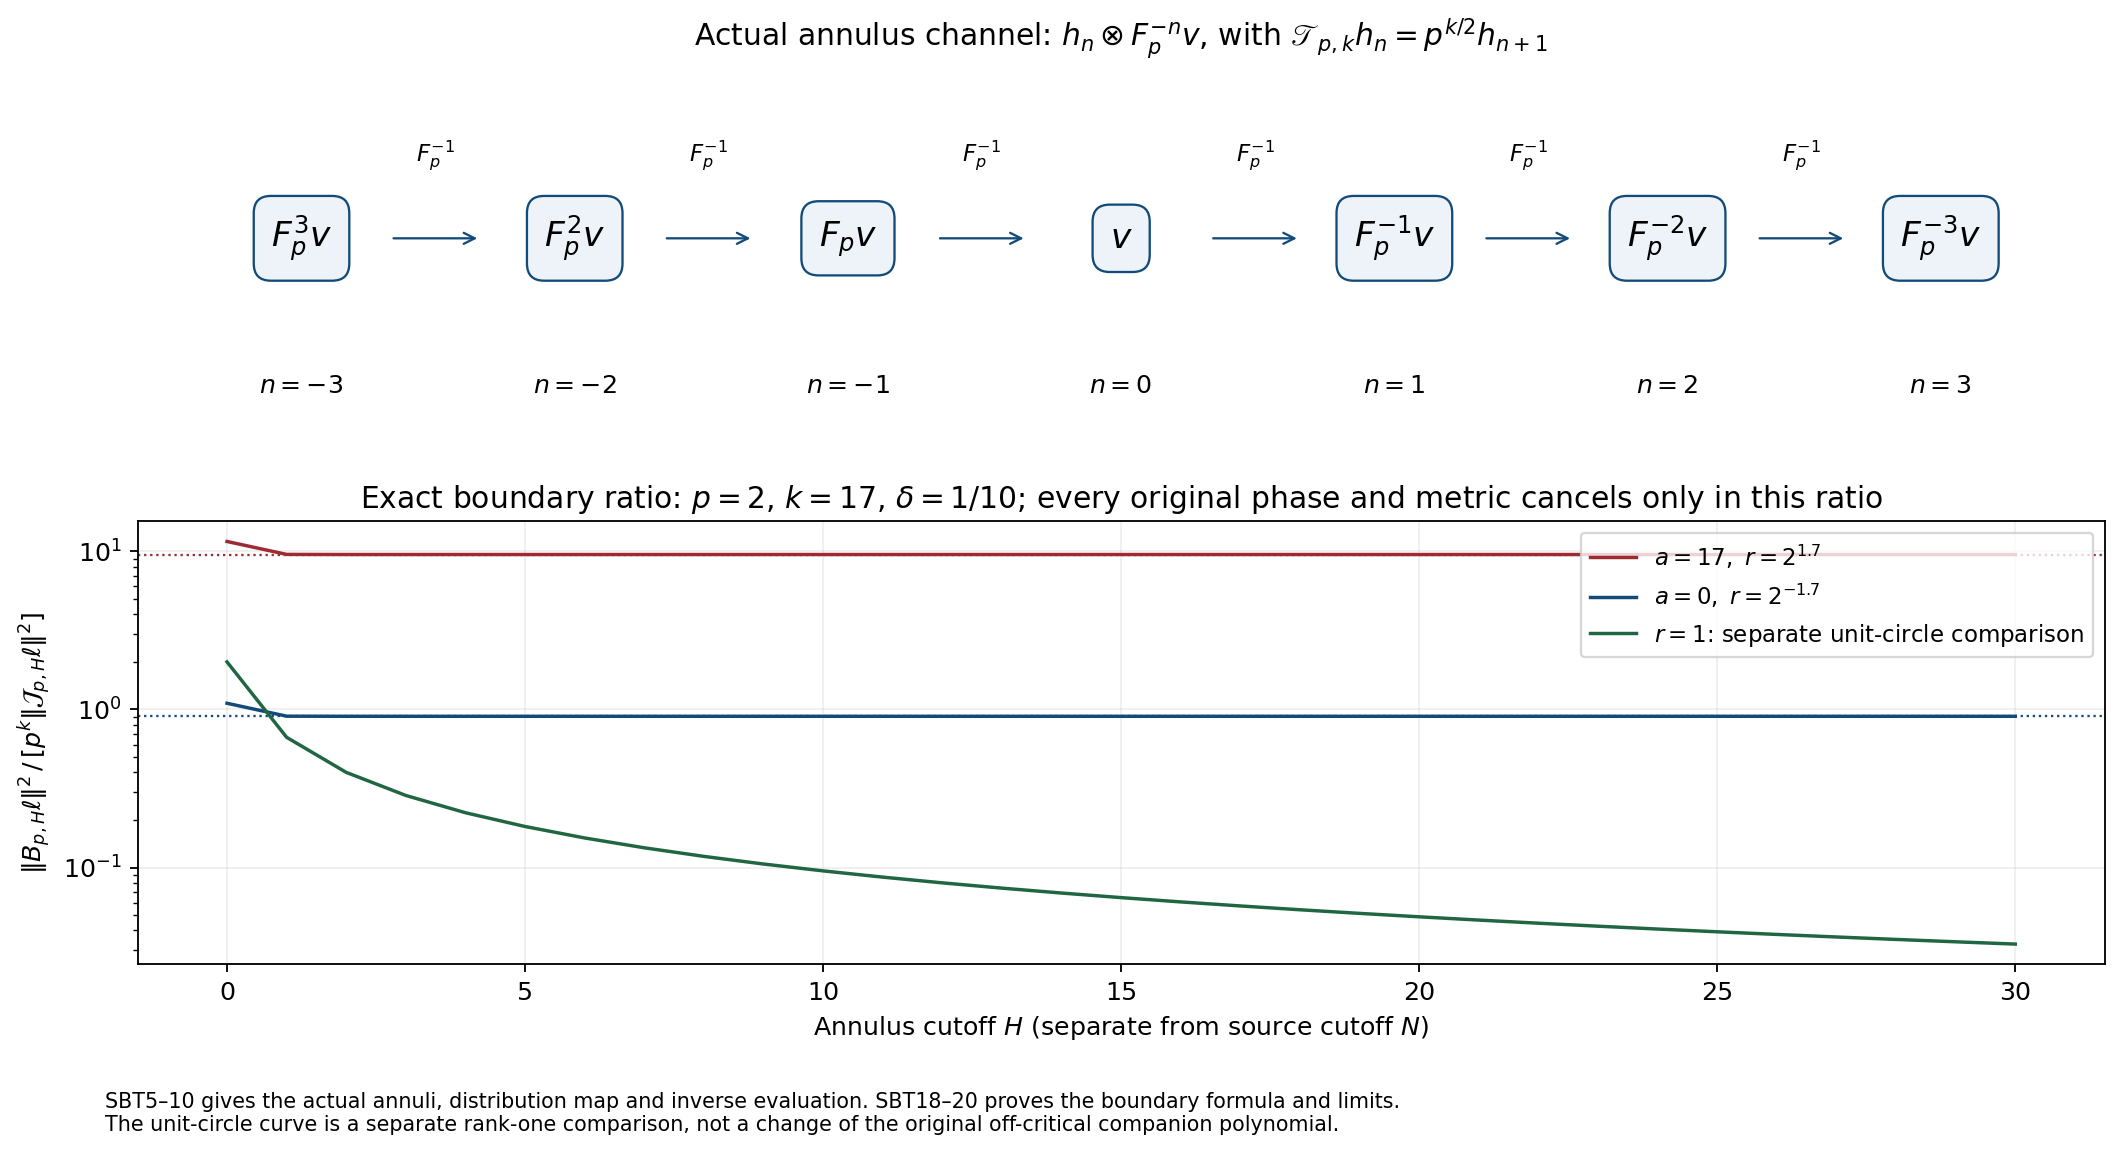
\includegraphics[width=\linewidth]{ANNULUS_BOUNDARY.png}
\caption{SBT5--10 constructs the actual annulus channel and its
original $E$-valued coefficient sequence. The arrows between
coefficients are $F_p^{-1}$; the spatial shift itself acts on $h_n$.
SBT18--20 proves the displayed boundary ratio and its nonzero
off-circle limits. The unit-circle curve is the separate comparison
explicitly defined after SBT15, not a modification of the original
off-critical polynomial. The inherited relative degree operator is
proved in PME1--5 and the supplied 031 PD1--21 source.}
\end{figure}
\end{document}
